\documentclass{scrartcl}
%\usepackage{german}
\usepackage[latin1]{inputenc}
\usepackage[german]{babel}

% zus�tzliche mathematische Symbole, AMS=American Mathematical Society 
\usepackage{amssymb}
\usepackage{amsmath}
\usepackage{booktabs}
\usepackage{float}
\usepackage{array}
\usepackage{subcaption}
\usepackage{xcolor}
\usepackage{hyperref}

% f�rs Einbinden von Graphiken
\usepackage{graphicx}

% f�r Namen etc. in Kopf- oder Fu�zeile
\usepackage{fancyhdr}

% erlaubt benutzerdefinierte Kopfzeilen 
\pagestyle{fancy}




% Definition der Kopfzeile
\lhead{
ICHaus Interpolationsplatine Anleitung
}
\chead{}
\rhead{\today{}}
\lfoot{}
\cfoot{Seite \thepage}
\rfoot{} 


\begin{document}


\begin{titlepage}
	\begin{center}
		\vspace*{1cm}
		
		\Huge
		\textbf{ICHaus Interpolationsplatine}
		
		\vspace{0.5cm}
		\LARGE
		Kurzanleitung
		
		\vspace{1.5cm}
		
		\textbf{S�ren Alrutz}
		
		\vfill
		
		Platine zum Wandeln von 1Vpp und 11$\mu$Ass Signalen zu 5V TLL Level
		
		\vspace{0.8cm}
		
		
		
		\Large
		\today
		
	\end{center}
\end{titlepage}


\section{Disclaimer}

Die Anleitung wurde nach bestem Wissen und Gewissen geschrieben, allerdings nicht sonderlich Intensiv auf sprachliche/Inhaltliche Fehler gepr�ft.
Die Platine wurde fast vollst�ndig nach Schaltpl�nen und Vorschl�gen des Datenblatts aufgebaut. Hier sind alle Information auch noch genauer erkl�rt. Schaltpl�ne und Layout sind auf meinen Github zu finden: \url{https://github.com/Shep-pard/ICHausInterpolation}

\section{Basics zum Verwendeten IC}

Die Platine basiert auf dem ICHaus IC-NV IC. Dies ist ein vollintegrierter 6 Bit Sin/Cos Interpolationschip. Durch die 6 Bit ist eine Aufl�sung von 64 Pulsen pro Periode m�glich. Dies entspricht einer 16-fachen Interpolation des sinusf�rmigen Signals.\\
Die Eingangssignale d�rfen bei maximaler Interpolation noch eine Frequenz von 200kHz haben. Bei niedrigeren Faktoren ist eine maximale Frequenz bis zu 320kHz m�glich. Das Referenzsignal des Eingangs kann �ber einen Komparator ausgegeben werden.

\section{Aufbau der Platine}

Abbildung \ref{fig:total} zeigt eine der Platinen von der Seite. An der unteren Seite sind die Steckverbinder. Es k�nnen jeweils sowohl 9 Pin D-Sub Buchsen als auch 2Pin 3,5mm Pitch Steckverbinder verwendet werden. Der linke Stecker ist der Eingang f�r Encoder/GMS. Der rechte Stecker geht an die Auswertung und versorgt die Platine mit 5V. Seitlich neben dem GMS Eingang ist noch ein weiterer 2 Pin Steckverbinder. Dieser ist zum Anschluss des Schirms des GMS gedacht wenn kein D-Sub Verbinder verwendet wird.


\begin{figure}[H]
	\begin{center}
		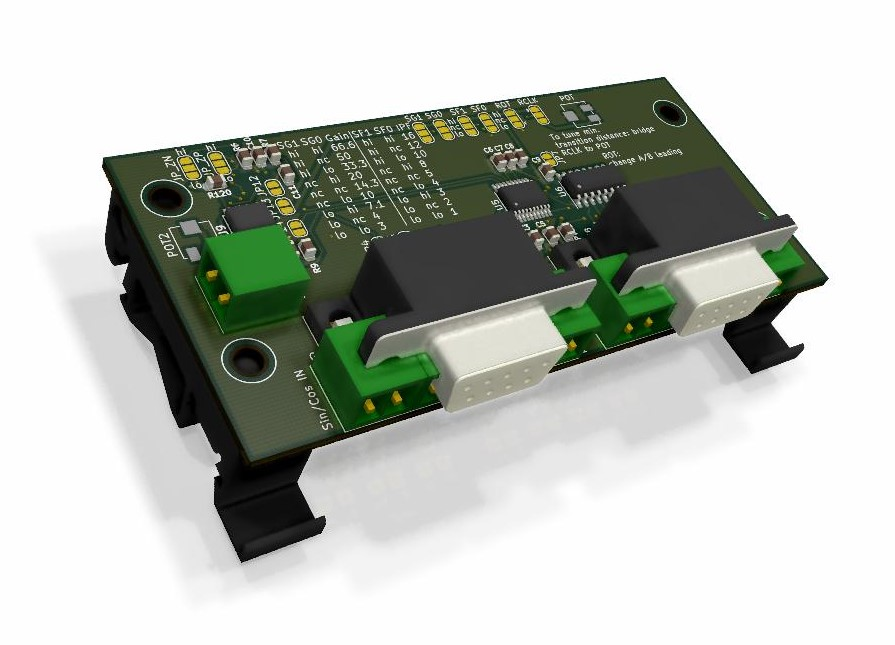
\includegraphics[width=0.8\textwidth]{total.jpg}
	\end{center}
	\caption{Gesamtansicht der Platine}
	\label{fig:total}
\end{figure} 


Des weiteren ist auf der Platine auf der linken Seite ein Operationsverst�rker zur Interpretation des Referenzimpuls verbaut. In der Mitte ist der IC-NV und rechts davon ein 4 Kanal Differentialtreiber um die Signale des IC-NV St�rungssicher auszugeben.



\section{Steckverbinder Pinout}

\subsection*{D-Sub}
Das Pinout der D-Sub Verbinder ist f�r beide fast identisch. Auf Tabelle \ref{tab:dsub} sind beide Pinouts aufgelistet. Der Unterschied ist nur der dedizierte Schirm Anschluss f�r den Encoder/GMS.

\begin{table}[h]
	\centering
	\caption{Pinout D-Sub 9 Verbinder}
	\label{tab:dsub}
	\begin{tabular}{c|ll}
		Pin &  TTL Output	& Encoder/GMS Eingang \\
		\midrule
		1 	&GND 			& Schirm\\
		2 	&Z- 				&Z-\\
		3 	&B- 				&B-\\
		4 	&A- 				&A-\\
		5 	&5V In				&5V Out\\
		6 	&GND				&GND\\
		7 	&Z+ 				&Z+\\
		8 	&B+ 				&B+\\
		9 	&A+ 				&A+
	\end{tabular}
\end{table}

\subsection*{3,5mm Schraubklemmen}

Zur Verdrahtung der Schraubklemmen ist jeder Pin auf der Platine einzeln beschriftet. Nur f�r den Schirm des Encoder/GMS Anschluss ist eine extra Schraubklemme vorhanden.\\
\textbf{Fehler bei der Beschriftung: Bei P5 steht neben "Schirm" f�lschlicherweise 5V und GND. Das kann ignoriert werden!}


\section{Platine Einstellen}
Die Platine ist standardm��ig f�r die Verwendung mit 11$\mu$Ass ausgelegt.

\begin{figure}[H]
	\begin{center}
		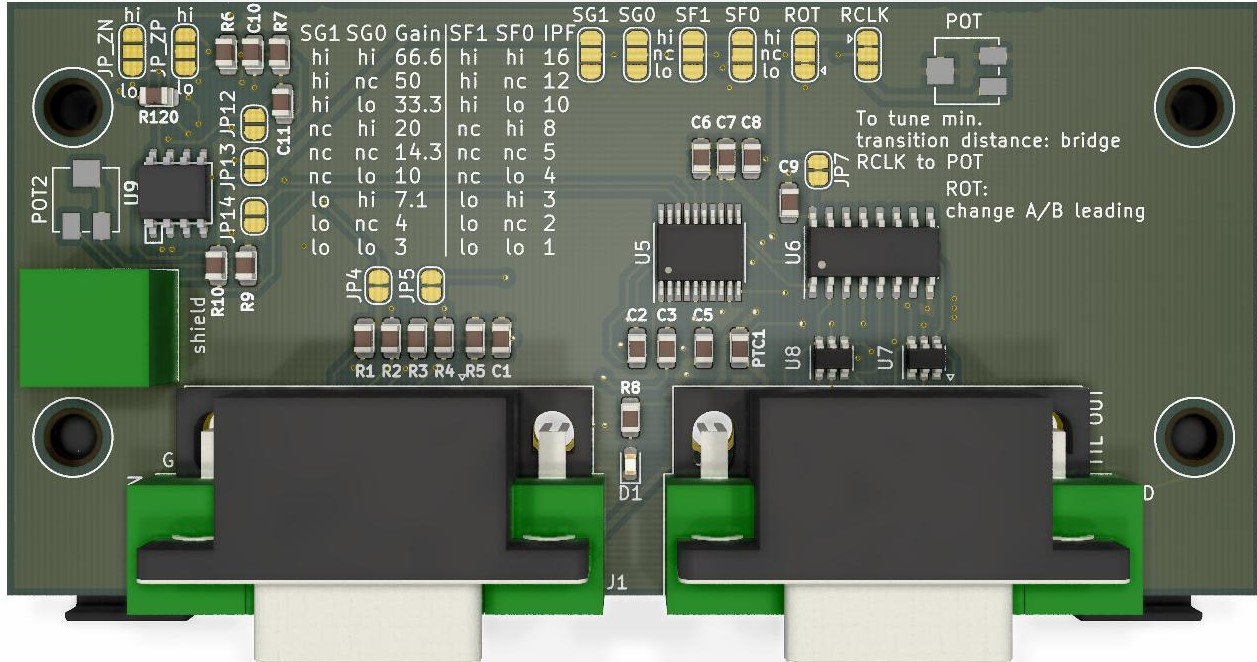
\includegraphics[width=0.8\textwidth]{top.jpg}
	\end{center}
	\caption{Top Ansicht der Platine}
	\label{fig:top}
\end{figure} 

\subsection*{11$\mu$Ass}

Zur Auswertung von 11$\mu$Ass Signalen m�ssen auf der Platine einige Grundvoraussetzungen erf�llt sein:
\begin{itemize}
	\item R1-R4 m�ssen 25k$\Omega$ sein
	\item JP2/JP3 offen 
	\item JP4/JP5 geschlossen
\end{itemize}

Um den Referenzimpuls auszuwerten muss zus�tzlich \textit{JP12} geschlossen sowie \textit{JP\_ZN} und \textit{JP\_VP} auf lo sein.

Der Gain kann auf zwischen 4 oder 7,1 mit den Jumpern \textit{SG0} und \textit{SG1} gestellt werden. Wenn das Ergebnis nicht zufriedenstellend ist, muss der Gain eventuell experimentell angepasst werden.


\subsection*{1VPP}

\begin{itemize}
	\item R2 und R4 m�ssen 120$\Omega$ sein
	\item JP2/JP3 geschlossen 
	\item JP4/JP5 geschlossen
\end{itemize}

Um den Referenzimpuls auszuwerten muss zus�tzlich \textit{JP12-JP15} offen sowie \textit{JP\_ZN} und \textit{JP\_VP} auf high sein.

Der Gain kann auf zwischen 3 oder 4 mit den Jumpern \textit{SG0} und \textit{SG1} gestellt werden. Wenn das Ergebnis nicht zufriedenstellend ist, muss der Gain eventuell experimentell angepasst werden.


\subsection*{Referenzsignal}

Das Referenzsignal des Encoder/GMS kann entweder ausgewertet werden oder es kann automatisch ein Impuls jede Periode erzeugt werden. F�r die automatische Signalerzeugung \textit{JP13/JP14} schlie�en.\\

\noindent
F�r die Auswertung muss das Poti POT2 korrekt eingestellt werden. Zur Erkl�rung sind auf Abbildung \ref{fig:1uass} die analogen Signale eines 11$\mu$Ass GMS abgebildet. Das Referenzsignal ist die rote Kurve unten. Das Poti ver�ndert das blaue Signal.
Zur Auswertung des Referenzimpuls ist sowohl das blaue als auch das rote Signal an einen Komperator angeschlossen. Wenn die rote Kurve �ber der blauen ist, wird in der Sinusperiode ein Referenzimpuls ausgegeben.


\begin{figure}[H]
	\begin{center}
		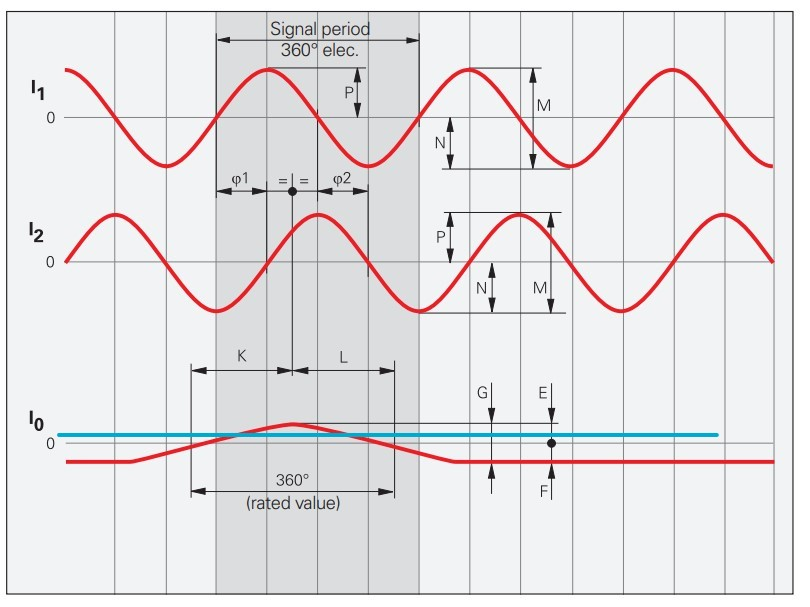
\includegraphics[width=0.8\textwidth]{11uass.jpg}
	\end{center}
	\caption{Analoge Signale von einem GMS}
	\label{fig:1uass}
\end{figure}

Um das Poti einzustellen, k�nnen die Spannungen entweder mit einem Oszilloskop gemessen und angepasst werden oder mit Hilfe von LinuxCNC ausgewertet werden. Zur Auswertung in LinuxCNC das Halscope �ffnen und Encoder A/B/Index Signale anzeigen und auf das Index Signal triggern. Immer �ber den Referenzimpuls fahren und das Poti einstellen bis nur noch ein Referenzimpuls angezeigt wird. Siehe Abbildung \ref{fig:linuxcnc}



\begin{figure}[H]
	\begin{center}
		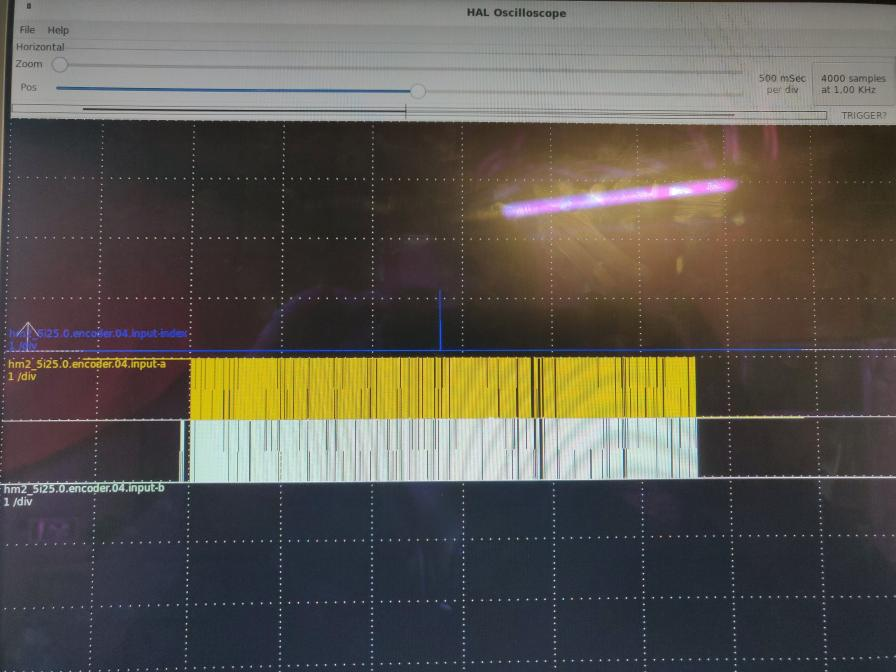
\includegraphics[width=0.8\textwidth]{linuxcnc.jpg}
	\end{center}
	\caption{Auswertung des Encoders/GMS in Linuxcnc}
	\label{fig:linuxcnc}
\end{figure}



\subsection*{Ausgangssignale}

Der Output der TTL Signale kann normal oder differentiell �bertragen werden. Standardm��ig wird ein differentielles Signal ausgegeben. Wenn dies nicht gew�nscht ist, muss mit einem Messer \textit{JP7} aufgetrennt werden und \textit{JP8-JP10} geschlossen werden.





\end{document}